Un edificio tiene 25 pisos de 8 departamentos cada uno.
La dueña del edificio ha definido una estrategia
para ponerle precio a cada departamento.

\begin{minipage}[T]{.71\textwidth}
  El número que identifica cada departamento se divide en dos partes:
  los dos últimos dígitos indican en qué posición está
  (de acuerdo al dia\-grama),
  y los restantes indican el piso.
  Por ejemplo, el departamento 1105 está en el undécimo piso,
  en la posición 5.
  \\[.6ex]
  Los dos departamentos al extremo derecho del diagrama
  tienen vista al mar,
  y los dos del extremo izquierdo
  tienen vista al cerro.
\end{minipage}
\hspace{1em}
\begin{minipage}[T]{.25\textwidth}
  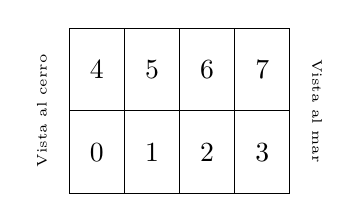
\begin{tikzpicture}[yscale=1.5, scale=.7]
    \draw (0, 0) grid (4, 2);
    \foreach\i in {0,...,3}
      \node at (+0.5 + \i, 0.5) {\i};
    \foreach\i in {4,...,7}
      \node at (-3.5 + \i, 1.5) {\i};
    \node[rotate=-90, font=\tiny] at ( 4.5, 1) {Vista al mar};
    \node[rotate=+90, font=\tiny] at (-0.5, 1) {Vista al cerro};
  \end{tikzpicture}
\end{minipage}

Todos los departamentos del primer piso valen 100,
y todos los departamentos del último piso valen 400.

Para los pisos intermedios,
se ha fijado un precio base de 245;
el precio de los departamentos con vista al mar se aumentará en 13\%,
y el de los con vista al cerro se rebajará en 17\%.
Los decimales se redondearán hacia abajo.

Adicionalmente,
se difundió el rumor de que el ídolo adolescente Justino Vivar
habría alojado una noche en el departamento 807.
Como hay un gran interés entre sus fanáticas
por adquirir este departamento,
la dueña ha decidido fijar su precio en 500.

Escriba un programa que pregunte al comprador el número del departamento,
y le entregue cuál es el precio de ese departamento.

